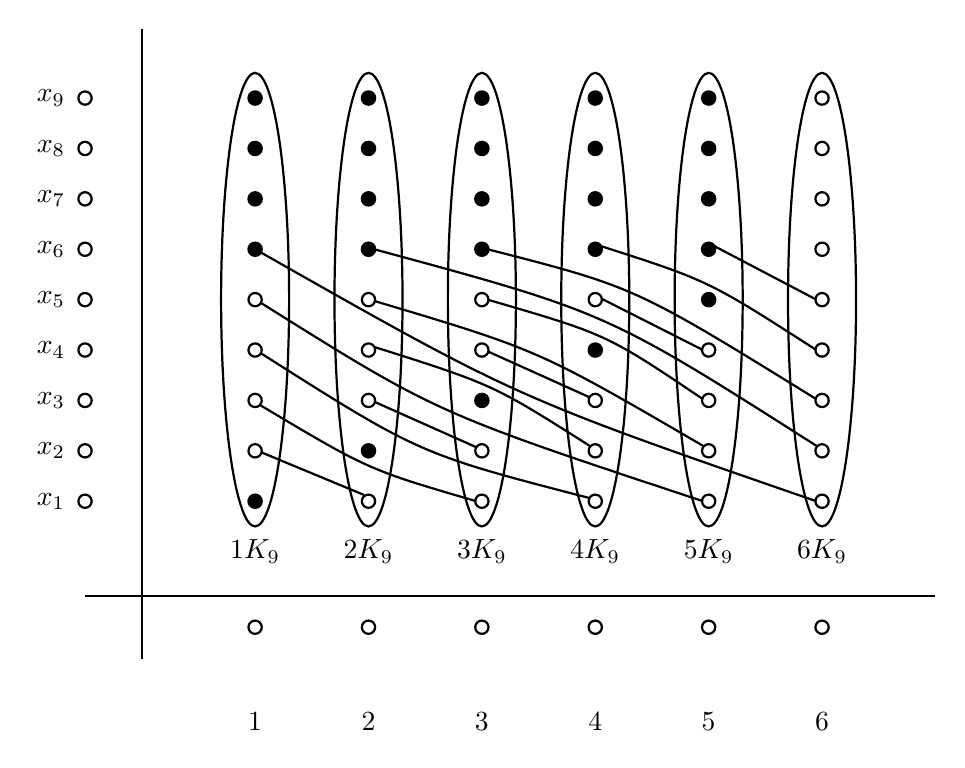
\begin{tikzpicture}[scale=0.8,thick,x=1.8cm,y=1cm]
\def\vr{3pt}

% axes
\draw (-0.5,-1.5) -- (7,-1.5);
\draw (0,-2.5) -- (0,7.5);

% left reference dots x_1,...,x_9
\foreach \k [count=\i from 0] in {x_1,x_2,x_3,x_4,x_5,x_6,x_7,x_8,x_9}{
  \draw (-0.5,0.8*\i) [fill=white] circle (\vr);
}
% left labels
\foreach \k [count=\i from 0] in {x_1,x_2,x_3,x_4,x_5,x_6,x_7,x_8,x_9}{
  \node at (-0.8,0.8*\i) {$\k$};
}

% bottom row reference dots under the axis
\foreach \i in {1,...,6}{
  \draw (\i,-2) [fill=white] circle (\vr);
  \node at (\i,-3.5) {$\i$};
}

% column 1 (1K_9)
\begin{scope}[yshift=0cm]
  \foreach \i/\c in {1/black,2/white,3/white,4/white,5/white,6/white}{
    \draw (\i,0) [fill=\c] circle (\vr);
  }
  \draw (1,3.2) ellipse (0.3 and 3.6);
  \node at (1,-0.8) {$1K_9$};
\end{scope}

% column 2 (2K_9)
\begin{scope}[yshift=0.8cm]
  \foreach \i/\c in {1/white,2/black,3/white,4/white,5/white,6/white}{
    \draw (\i,0) [fill=\c] circle (\vr);
  }
  \draw (2,2.4) ellipse (0.3 and 3.6);
  \node at (2,-1.6) {$2K_9$};
\end{scope}

% column 3 (3K_9)
\begin{scope}[yshift=1.6cm]
  \foreach \i/\c in {1/white,2/white,3/black,4/white,5/white,6/white}{
    \draw (\i,0) [fill=\c] circle (\vr);
  }
  \draw (3,1.6) ellipse (0.3 and 3.6);
  \node at (3,-2.4) {$3K_9$};
\end{scope}

% column 4 (4K_9)
\begin{scope}[yshift=2.4cm]
  \foreach \i/\c in {1/white,2/white,3/white,4/black,5/white,6/white}{
    \draw (\i,0) [fill=\c] circle (\vr);
  }
  \draw (4,0.8) ellipse (0.3 and 3.6);
  \node at (4,-3.2) {$4K_9$};
\end{scope}

% column 5 (5K_9)
\begin{scope}[yshift=3.2cm]
  \foreach \i/\c in {1/white,2/white,3/white,4/white,5/black,6/white}{
    \draw (\i,0) [fill=\c] circle (\vr);
  }
  \draw (5,0) ellipse (0.3 and 3.6);
  \node at (5,-4) {$5K_9$};
\end{scope}

% column 6 (6K_9)
\begin{scope}[yshift=4cm]
  \foreach \i/\c in {1/black,2/black,3/black,4/black,5/black,6/white}{
    \draw (\i,0) [fill=\c] circle (\vr);
  }
  \draw (6,-0.8) ellipse (0.3 and 3.6);
  \node at (6,-4.8) {$6K_9$};
\end{scope}

% extra stacked layers (matching the original appearance)
\begin{scope}[yshift=4.8cm]
  \foreach \i/\c in {1/black,2/black,3/black,4/black,5/black,6/white}{
    \draw (\i,0) [fill=\c] circle (\vr);
  }
\end{scope}

\begin{scope}[yshift=5.6cm]
  \foreach \i/\c in {1/black,2/black,3/black,4/black,5/black,6/white}{
    \draw (\i,0) [fill=\c] circle (\vr);
  }
\end{scope}

\begin{scope}[yshift=6.4cm]
  \foreach \i/\c in {1/black,2/black,3/black,4/black,5/black,6/white}{
    \draw (\i,0) [fill=\c] circle (\vr);
  }
\end{scope}

% inter-column edges (as in the original image)
\draw (1.05,0.78) -- (1.96,0.1);
\draw (1.05,1.52) .. controls (2,0.5) .. (2.95,0);
\draw (1.05,2.35) .. controls (2.45,0.75) .. (3.95,0.05);
\draw (2.05,1.58) -- (2.96,0.85);
\draw (1.05,3.15) .. controls (2.6,1.4) .. (4.95,0);
\draw (2.05,2.45) .. controls (3.1,1.85) .. (3.95,0.88);
\draw (1.05,3.95) .. controls (3.3,1.65) .. (5.95,0);
\draw (3.05,2.38) -- (3.95,1.65);
\draw (2.05,3.18) .. controls (3.5,2.4) .. (4.95,0.88);
\draw (3.05,3.2) .. controls (4.1,2.65) .. (4.95,1.62);
\draw (2.05,4) .. controls (4.1,3) .. (5.95,0.88);
\draw (4.05,3.22) -- (4.95,2.4);
\draw (3.05,4) .. controls (4.35,3.4) .. (5.95,1.62);
\draw (4.05,4.05) .. controls (5,3.5) .. (5.95,2.4);
\draw (5.05,4.05) -- (5.95,3.2);

\end{tikzpicture}